\documentclass[12pt,oneside]{report}
\usepackage[margin=1in]{geometry}
\usepackage{setspace}
\usepackage{longtable}
\usepackage{supertabular}
\usepackage{afterpage}

\usepackage[sort]{natbib}
\bibliographystyle{sb}
    \bibpunct[:]{(}{)}{;}{a}{}{,}
\usepackage[colorlinks=false,hidelinks]{hyperref}

\usepackage{doi}

\usepackage{amsmath,amssymb}
\usepackage{booktabs}
\usepackage{array}
\usepackage{graphicx}
\usepackage{xspace}

\graphicspath{{graphics/}}

\input{localpackages.tex}


\title{Do Styles Make Fights?}
\author{Jarvis Xie}

\begin{document}
\thispagestyle{empty}
\begin{titlepage}
    \begin{center}
        \vspace*{0pt}
        \makeatletter
        \Huge
        \textbf{\@title}\\
        \vspace{1ex}
        \Large
        Data-Driven Style Discovery, Outcome Prediction, and Upset Detection in the UFC \\
        \vspace{5ex}
        \textbf{Jarvis Xie}\\
        \vspace{.5ex}
        Advisor: Robert Wooster
        \vfill
        \large\textit{Submitted to the faculty of the Department of Statistics \& Data Science\\in partial fulfillment of the requirements for the degree of Bachelor of Arts}\\
        \vspace{3ex}
        
\includegraphics[width=0.275\textwidth]{graphics/yale-crest.png}\\
        \vspace{2ex}
        \large
        \textsc{Department of Statistics \& Data Science}\\
        \textsc{Yale University}\\
        \vspace{.5ex}
        \normalsize \today\\
        \makeatother
    \end{center}

    \newpage

    \thispagestyle{empty}
    { }
\end{titlepage}


% =====================================================================
\chapter*{Abstract}
\thispagestyle{empty}
% =====================================================================

``Styles make fights'' is the most-repeated cliché in mixed martial
arts.  Most statistical models of UFC outcomes do not encode style
explicitly: they feed per-minute striking and grappling rates, physical
covariates, and experiential covariates into supervised classifiers, and whatever
residual structure style contributes is left to the classifier to
exploit.  This thesis asks three questions of that cliché---whether
latent fighting styles, recovered from career-level fighter profiles,
sharpen our predictions of who wins, how the fight
unfolds, and when a favorite is vulnerable.

Using a unified matchup-level table built from UFC fight data and
containing $8{,}482$ event-ordered rows through 2024 (Section~\ref{sec:repro}), we learn soft
Gaussian mixture posteriors and an autoencoder
embedding in \(\mathbb{R}^3\) from career-level fighter profiles, attach them as
matchup descriptors, and evaluate downstream
models on an event-ordered held-out test slice.  The answers to the
three questions differ sharply in kind.  For who wins, style
is a marginal contributor: a Vegas-aware LR$+$HGB$+$RF stack edges the de-vigged Vegas baseline on
AUC, Brier, and log loss once \(p_{\mathrm{vegas},A}\) is added as a meta-input, with paired-bootstrap confidence intervals
excluding zero, but the effect is small and the same stack without Vegas
is strictly worse than Vegas.  For how the fight
unfolds, style is a first-class signal: top-quintile \(K = 5\)
GMM-posterior style divergence sits roughly nine percentage points above the middle bins in realized finish rate, and a hierarchical method-of-victory factorization
cuts six-way log loss by about ten percent.  For when a
favorite is vulnerable, the autoencoder embedding is the largest
non-market contributor to a residual upset detector; an exploratory de-vigged
flat-stake ROI simulation produces a positive return at post-hoc \(\theta = 0.15\) on a single
held-out slice, providing evidence of residual market information
rather than a deployable betting strategy.  Style helps least where
MMA analysts most often invoke it (who wins) and most where they
rarely do (how fights unfold and where the market is wrong); the
results should be read with the caveats on data, market access, and
threshold selection set out in Chapters~\ref{ch:upset}
and~\ref{ch:conclusion}.

\newpage
\pagenumbering{roman}

\addtocontents{toc}{\vspace{0pt}\protect\noindent\parbox[t]{\textwidth}{\normalsize\textcolor{black}{\textbf{Front matter}}}\par}

\singlespacing
\setstretch{0.95}
\tableofcontents
\setstretch{1}

\clearpage\chapter*{Acknowledgments}\addcontentsline{toc}{section}{Acknowledgements}

I am grateful to my advisor, Professor Robert Wooster, for his
guidance, and to the Yale Department of Statistics and Data Science
for the framework that made this work possible.  Every empirical
result depends on the UFCStats scrape and the Kaggle community odds
datasets \citep{ufckagglealibi,ufcoddskaggle}.

\normalsize
\newpage
\pagenumbering{arabic}
\onehalfspacing
\setlength{\parindent}{1.5em}


% =====================================================================
\chapter{Introduction}\label{ch:introduction}
% =====================================================================

``Styles make fights'' is the most-quoted cliché in mixed martial
arts.  Broadcasters explain outcomes through the language of
archetypes---striker against grappler, pressure fighter against
counter-puncher---and attribute results to the stylistic pairing
rather than to raw quality.  Statistical work on UFC outcomes has been
slow to encode this intuition.  The standard pipeline feeds per-minute striking rates, takedown accuracy, control time,
physical attributes, and recent form into supervised classifiers
\citep{hitkul2019mma,yin2024mma,sheng2024ufc}; each
feature enters as an independent input and whatever structure
``style'' contributes is left to the downstream classifier to
discover implicitly.  When style does enter explicitly, it does so
through hand-applied labels---``striker,'' ``grappler,''
``hybrid''---that analysts disagree about and that cannot represent
continuous variation in fighting behavior.  This thesis asks whether
latent fighting styles can instead be recovered from career-level
fighter profiles, and whether, once recovered, they sharpen our
predictions of who wins a fight, how the fight unfolds,
and when a favorite is vulnerable.

The three questions are ordered by the difficulty with which they can
be answered in the affirmative.  Predicting wins in a combat sport
with a roughly $55\%$ finish rate and large fighter-to-fighter
variance is hard, and the betting market already integrates much
public and private information.  Predicting how a fight unfolds is a
richer task with more outcome categories in which style can leave a
fingerprint.  Identifying upsets is a narrower residual task if genuine style
effects are concentrated in the tails of mismatched matchups---where
a favorite looks dominant by every numeric feature but is
stylistically exposed.  The rest of the thesis finds that this
ordering is the right one.

Two methodological points shape how the empirical chapters should be
read.  First, the style features---Gaussian mixture posteriors, the
Hybrid Score, the autoencoder embedding, and the empirical
style-pair heatmap---are derived from career-aggregate
fighter profiles fitted once on the full corpus, and serve as
retrospective descriptors of fighter identity rather than strict
pre-fight predictors; the matchup-level rolling rates, Elo, and
Glicko-2 ratings are walked chronologically and are the
prospectively defensible block.  Section~\ref{sec:leakage-scope}
states this scope explicitly.  Second, the comparisons in
Chapter~\ref{ch:matchup} are run on two distinct test slices---the
full event-ordered test fold and a smaller Vegas-aligned subset---and
we are careful in the tables to distinguish ``feature gain'' from
``subset change.''

The empirical headline runs as follows.  For who wins, a
non-market feature ablation across six model families lifts held-out AUC from
$0.600$ to $0.670$ over a $Z$-score-delta baseline, and a
Vegas-aware LR$+$HGB$+$RF stack edges the de-vigged Vegas baseline on
AUC, Brier, and log loss once \(p_{\mathrm{vegas},A}\) is added as a
meta-input.  For how fights unfold, top-quintile \(K = 5\)
GMM-posterior style divergence sits roughly nine percentage points above the middle bins in realized finish rate, and a hierarchical method-of-victory decomposition cuts
six-way log loss.  For when a favorite is vulnerable, a
Vegas-aware residual upset model in which the autoencoder embedding
is the single largest non-market contributor produces an exploratory de-vigged
flat-stake ROI whose paired-bootstrap $95\%$ CI excludes zero at post-hoc \(\theta = 0.15\) on a
single held-out window.  Style, in short, helps make fights, but
in a more specific sense than the cliché usually conveys: it helps
least where MMA analysts most often invoke it (who wins) and most
where they rarely do (how fights unfold and where the market is wrong).

% =====================================================================
\chapter{Background and Related Work}\label{ch:background}
% =====================================================================

The peer-reviewed literature on supervised UFC outcome prediction
is small.  \citet{hitkul2019mma} present an early comparative study
that evaluates random forests \citep{breiman2001random}, decision
trees, a perceptron, stochastic-gradient-descent logistic regression,
support vector machines, and $k$-nearest neighbors on a UFC scrape,
reporting roughly $63\%$ accuracy on a random hold-out.  More
recently, \citet{sheng2024ufc} benchmark random forests, gradient
boosted decision trees, and SVMs on the Kaggle ``UFC-Master'' dataset
and identify age difference and fight date as their most influential
features.  Closest in spirit to the present work,
\citet{yin2024mma} applies factor analysis to per-fight statistics,
clusters fighters into a handful of technical styles with $k$-means,
and feeds the style assignment into an ensemble of logistic regression,
random forest, SVM, XGBoost \citep{chen2016xgboost}, and a shallow
neural network, reaching $65.5\%$ accuracy and showing in an ablation
that the style factor contributes positively.  None of these studies
use a chronological split, a calibrated probabilistic baseline, or a
continuous style embedding, and none compare their predictions to
market odds.  On the unsupervised style side,
\citet{hackett2017mma} model MMA fighters as mixtures of ten
data-defined prototypical martial arts styles.  Their mixed-membership
approach is an important precedent for treating fighting style as a
learned latent object rather than a hand label.  The present thesis
differs by learning GMM posteriors and an autoencoder embedding from
UFCStats career profiles, attaching those descriptors to a
chronologically evaluated UFC prediction pipeline, and testing their
role in winner prediction, fight dynamics, and Vegas-residual upset
detection.  A recurring pitfall across the body of work is
data leakage: career-aggregate features computed on the full
dataset yield optimistically biased test metrics when the aggregation
window includes the fight being predicted.  The present thesis
distinguishes its features by leakage scope: rolling pre-fight
rates and Elo/Glicko-2 ratings are walked in strict chronological
order (Chapter~\ref{ch:data}), while the style features
(Chapter~\ref{ch:style}) are static career-aggregate descriptors
fitted once on the full corpus.  Section~\ref{sec:leakage-scope}
spells out exactly which columns are which, and how that distinction
shapes the interpretation of every downstream result.

Two rating systems appear as features throughout.  Elo
\citep{elo1978rating} updates each competitor after every bout based
on the actual versus expected outcome; the rating difference, passed
through a logistic CDF, yields a win probability.  Glicko-2
\citep{glickman1999parameter,glickman2012example} extends Elo with a
rating deviation and a volatility term and behaves better for
fighters with layoffs or small samples.  Both are walked
chronologically, so the rating used to predict a fight is strictly
the rating before it resolves.

For style discovery we use two complementary representations.
Gaussian mixture models
\citep{bishop2006pattern,hastie2009elements,dempster1977em} are the
soft-clustering counterpart of $K$-means: each fighter is associated
with a posterior \(\pi = (\pi_1, \ldots, \pi_K)\) over components
rather than a hard label, so hybrid fighters are represented by a
spread posterior rather than by an arbitrary hard assignment; the
Shannon entropy \(H(\pi) = -\sum_k \pi_k \log \pi_k\) summarizes stylistic hybridity in a single scalar (the Hybrid Score).
A feed-forward autoencoder \citep{hinton2006reducing} implemented in
PyTorch \citep{paszke2019pytorch} and optimized with Adam
\citep{kingma2014adam} embeds each qualified fighter into
\(\mathbb{R}^3\); differences and means of the two corners' embeddings
enter downstream models as matchup features.  Mixture posteriors
and a low-dimensional autoencoder solve different problems: the
mixture compresses each fighter into a soft membership over a small
set of archetypes, while the autoencoder supplies a smooth
\(\mathbb{R}^3\) space in which two fighters with the same hard
archetype can still sit far apart.  Chapter~\ref{ch:style} returns
to this distinction; Chapter~\ref{ch:upset} shows that for upset
detection the continuous embedding is doing nearly all of the style
work.  Within that precedent, the specific combination of GMM posteriors, continuous
autoencoder embeddings, chronological UFC outcome evaluation, and
Vegas-residual upset testing used here has not been studied to our knowledge.

Downstream, probability calibration matters whenever a model is used
for betting or resource allocation.  We use isotonic regression
\citep{zadrozny2002transforming,niculescu2005predicting} as a
post-hoc calibrator on individual models and on the stacked ensemble output; the stacked ensemble itself uses a logistic meta-learner over selected base-model probabilities \citep{wolpert1992stacked,breiman1996stacked};
calibration quality is reported as expected calibration error
\citep{guo2017calibration} alongside the Brier score
\citep{brier1950verification}.  For significance testing on paired
metrics we use the nonparametric paired bootstrap
\citep{efron1979bootstrap}, which yields percentile CIs and two-sided
$p$-values without parametric assumptions.  For interpretability we
report grouped permutation importance
\citep{breiman2001random} over semantic
feature families---rolling rates, style posteriors, embeddings,
ratings, physicals, Vegas---shuffling an entire group rather than
individual columns, which is more legible than SHAP when group
members are colinear.  All pipelines are implemented in scikit-learn
\citep{scikitlearn2011}, with XGBoost \citep{chen2016xgboost} and
LightGBM \citep{ke2017lightgbm} used where noted.

% =====================================================================
\chapter{Data and Preprocessing}\label{ch:data}
% =====================================================================

\section{Data sources}

The primary dataset is the UFC Fights, Fighters, and Events
Kaggle scrape of UFCStats \citep{ufcstats,ufckagglealibi}: fight-level
metadata (date, method, round, duration), per-fight positional
striking and grappling statistics, and fighter-level attributes
(date of birth, height, reach, stance, weight class).  After
cleaning, the merged fight-level scrape contains on the order
of seven thousand distinct UFC bouts from 1993 through 2024; all
supervised results in later chapters instead use a single
matchup-level feature table of $8{,}482$ event-ordered rows
($4{,}846{+}1{,}786{+}1{,}850$ train/validation/test;
Section~\ref{sec:repro}).  For the Vegas baselines we use a
community-maintained betting-odds Kaggle dump
\citep{ufcoddskaggle}, which contains both moneylines and
six-way method-of-victory props (KO/SUB/DEC for each corner).
Moneyline rows are filtered to US books and one row per fight
(latest \texttt{adding\_date}), with de-vigged implied probabilities
\(p_{\mathrm{vegas},A} = o_A^{-1} / (o_A^{-1} + o_B^{-1})\).
Method-of-victory probabilities are constructed as
$p_k = o_k^{-1}/\sum_{k'} o_{k'}^{-1}$ over the six method buckets,
i.e.\ proportional de-vigging across the multinomial outcome; the
binary \(p_{\mathrm{finish}}^{\mathrm{vegas}}\) used in
Chapter~\ref{ch:dynamics} is the sum of the four KO and SUB cells.
The moneyline and method-prop columns come from the same Kaggle dump, but completeness differs after cleaning and merging.  Thus the Vegas win-loss subset (\(n = 1{,}129\) on test) is not a superset of the finish-Brier subset (\(n = 1{,}827\)): some rows retain complete method prices even when the curated moneyline join fails, while some moneyline rows lack usable method fields.  Every Vegas-using analysis below names its subset.

\section{Pre-fight feature construction}

The matchup-level pipeline is built around a rolling pre-fight
aggregator that snapshots each fighter's cumulative career averages
before incorporating the current bout.  Output columns include
pre-fight per-minute rates (significant strikes, takedowns,
submission attempts, control ratio, positional striking shares), KO
and submission rates for and against, and five-fight recent form.
Because the aggregates at fight $t$ strictly exclude fight $t$ and
all subsequent fights, rolling columns are never contaminated by the
outcome they are used to predict---a common source of optimistic bias
in MMA prediction models.  Per-minute rates are
$Z$-scored within weight class to remove division-specific
baselines.  Elo ratings are walked with a standard specification
(initial $1500$, $K = 32$, logistic scale $400$;
\citealp{elo1978rating}) and Glicko-2 with monthly rating periods and
\(\tau = 0.5\) \citep{glickman2012example}; pre-fight $(R_A, R_B)$,
their difference, and Glicko-2 rating deviations are attached as
features.

A single artifact, \texttt{ufc\_matchup\_features.csv}, gathers every
column used downstream: identifiers, rolling rates for both corners
plus $\delta$ and $\mu$ transforms, \(K = 3\) and \(K = 5\) GMM
posteriors and Hybrid Scores, the three-dimensional autoencoder
embedding, physicals and weight-class one-hots, Elo and Glicko-2
ratings, an empirical style-pair heatmap probability
\(p_{\mathrm{heatmap},A}\) (the marginal \(K = 5\) cluster-pair win rate
described in Section~\ref{sec:heatmap}), and \(p_{\mathrm{vegas},A}\)
where available.  A \texttt{split} column $\in \{\text{train},
\text{val}, \text{test}\}$ from an event-ordered $60/20/20$ cut
ensures every downstream model shares the same training, validation,
and test events.  Every training row is augmented with its A/B
mirror so models cannot exploit the arbitrary corner convention, and
test metrics are reported on unmirrored rows so each fight counts
once.

\section{Leakage scope and feature blocks}\label{sec:leakage-scope}

Not every column in \texttt{ufc\_matchup\_features.csv} is
prospective in the strict pre-fight sense.  We group the columns
into three blocks and label each explicitly:

\begin{itemize}
\item \textbf{Pre-fight (chronologically walked).}  The rolling
career means \texttt{A\_pre\_*}, \texttt{B\_pre\_*},
\texttt{delta\_pre\_*}, the recent-five summaries, the Elo and
Glicko-2 rating columns, and the matchup transforms of these.  At
fight $t$ these columns use only fights strictly before $t$.

\item \textbf{Career-aggregate (retrospective).}  The GMM posteriors
\(\pi^{(K = 3)}\) and \(\pi^{(K = 5)}\), the Hybrid Score \(H(\pi)\), the
hard \(K = 5\) cluster assignment, the autoencoder embedding \(z\in \mathbb{R}^3\), the within-weight-class $Z$-scored rate columns
\texttt{*\_Z}, and the style-pair heatmap probability
\(p_{\mathrm{heatmap},A}\).  These are computed once from the
fighter-level table of career aggregates produced by notebook~05;
they are static fighter-level (or cluster-pair) descriptors and at
fight $t$ they reflect each fighter's full UFC career, not only the
fights before $t$.

\item \textbf{Concurrent.}  \(p_{\mathrm{vegas},A}\) is the de-vigged
moneyline implied probability at fight time and is by construction
pre-fight; the method-of-victory implied probabilities used in
Chapter~\ref{ch:dynamics} are likewise pre-fight market quantities.
\end{itemize}

The static block matters most for Chapter~\ref{ch:style}'s style
discovery (which is a description of fighter identity and is
naturally pooled across the career) and for downstream models that
use the style block as a covariate.  The cleanest way to read those
downstream results is therefore as evidence that fighter style,
as captured by a stable career-level summary, carries
predictive information about future fight outcomes; the full
strict-pre-fight version of the style features---refit on
expanding-window or rolling pre-fight statistics so that each
fighter's embedding at time $t$ uses only fights $<t$---would be the
deployable extension, which we leave to follow-up work.  The
case-study chapter (Chapter~\ref{ch:cases}) does refit the
supervised model prospectively for each historical event,
but the style features it pulls in remain static.

Two further design choices are deliberate.  The mirrored rows in
the training set keep models from learning a corner convention; the
unmirrored rows in test make every fight count once.  The
fighter-level cluster and embedding tables are not split because
Chapter~\ref{ch:style} is a retrospective description of fighter
identity rather than a new-fighter generalization experiment.
Refitting the representation on an expanding pre-fight window would
answer the stricter deployability question; here,
Section~\ref{sec:leakage-scope} clarifies that the static style
features should be read as career-level descriptors, not as features
known prospectively at every fight date.

\section{Reproducibility and selection discipline}\label{sec:repro}

\paragraph{Code and data.}  Analysis notebooks, feature-table construction, and bootstrap scripts are available at \url{https://github.com/Jaaxe/ufc-matchup-dynamics} (see also \texttt{README.md} and \texttt{run\_pipeline.py} in the repository root).

\paragraph{Splits.}  An event-ordered $60/20/20$ cut produces
$4{,}846$ train rows, $1{,}786$ validation rows, and $1{,}850$
test rows at the matchup-table level.  Restricting to rows with
de-vigged moneylines yields a Vegas-aligned test subset of $1{,}129$
rows; separately restricting to rows with the full six-way
method-of-victory market yields $1{,}827$ test rows for the
finish-Brier comparison in Chapter~\ref{ch:dynamics}.

\paragraph{What is fit on what.}  The fighter-level GMM, autoencoder,
and the \(K = 5\) heatmap are fit once on the static career
table, with the leakage caveat in Section~\ref{sec:leakage-scope}.
For each supervised model in Chapters~\ref{ch:matchup}--\ref{ch:upset},
hyperparameters and family choices are tuned on \texttt{val} (paired
five-fold walk-forward CV inside \texttt{train} where applicable),
isotonic calibration is fit on \texttt{val}, and \texttt{test} is
evaluated once.

\paragraph{What is selected after seeing test.}  Two choices were
made after looking at test outputs and we flag them as exploratory.
First, the upset threshold \(\theta = 0.15\) in
Chapter~\ref{ch:upset}'s ROI simulation is the smallest grid value
at which the bootstrap CI excludes zero; the table reports a grid
$\{0.05, 0.10, 0.15, 0.20\}$ but the headline number depends on
\(\theta = 0.15\) being the chosen threshold.  Second, the
case-study panel of Chapter~\ref{ch:cases} is a curated list of
five famous historical upsets---selected by canonical fame, not by
residual rank---and is presented as illustrative rather than as a
formal validation set.

\paragraph{Anchor figure.}  Figure~\ref{fig:matchup-corr} anchors
what follows.  Across the matchup table, significant-strike-volume
delta is the strongest raw correlate of the outcome
($\rho \approx 0.19$); reach and height deltas carry weaker signal
($\rho \approx 0.07$ and $0.03$); and a naïve hand-engineered
``style clash'' score correlates at essentially zero with who wins.
This foreshadows the thesis's central pattern: style will matter
more for how a fight unfolds than for the top-line outcome.

\begin{figure}[ht]
\centering
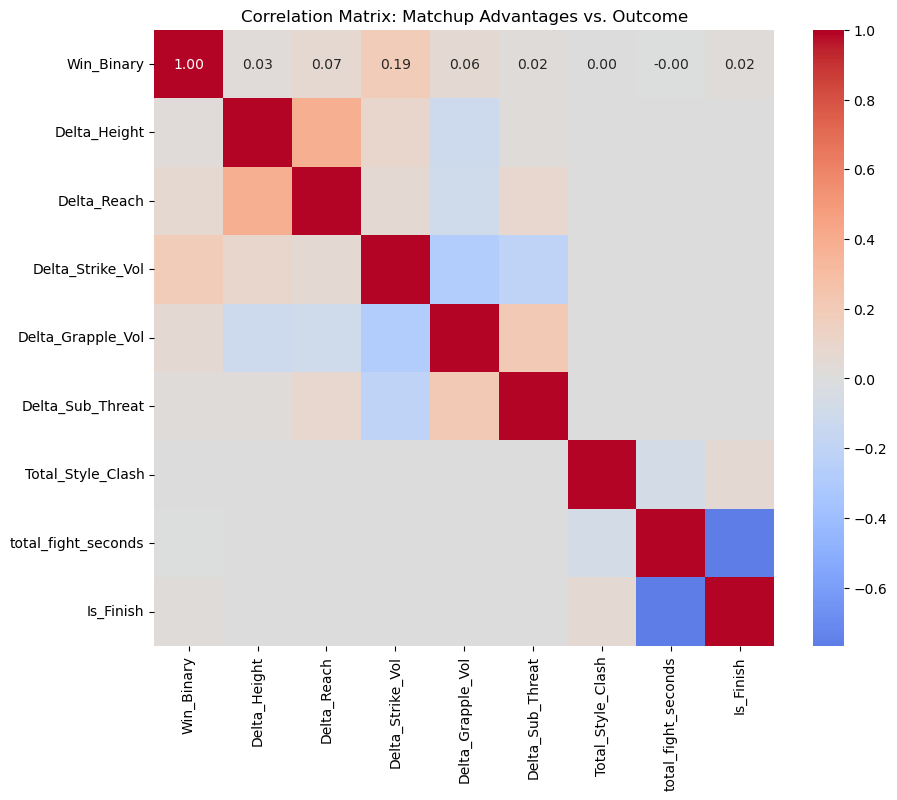
\includegraphics[width=0.70\textwidth]{matchup_correlation.png}
\caption{Matchup-level correlation matrix of A$-$B deltas with the
win and finish indicators.  Strike-volume delta is the largest raw
correlate of winning ($\rho = 0.19$); the ``style clash'' score is
near zero with the outcome; Chapter~\ref{ch:dynamics} shows that style divergence is more informative for finish and method than for the top-line winner.
Source: notebook~07.}
\label{fig:matchup-corr}
\end{figure}

% =====================================================================
\chapter{Discovering Fighting Styles}\label{ch:style}
% =====================================================================

Style discovery operates on a fighter-level profile \(x \in \mathbb{R}^7\) summarizing each qualified fighter's career: the
$Z$-scored per-minute rates of significant strikes, takedown
attempts, and submission attempts, the control-time ratio, and the
three positional shares of striking (distance, clinch, ground).
These seven features were chosen to isolate fighting behavior rather than fighter quality: they cover striking activity, grappling initiative, submission threat, control, and positional mode of engagement while excluding ratings, physical attributes, odds, and outcome variables.
Fighters with fewer than five UFC bouts are excluded because career-level per-minute rates are highly unstable at very small sample sizes; five fights is a practical cutoff that reduces one-fight noise while preserving enough fighters for clustering.  The same seven features feed all three
representations below---$K$-means, Gaussian mixtures, and an
autoencoder---so that any difference between representations reflects
model choice rather than feature engineering.

As stated in Section~\ref{sec:leakage-scope}, the GMM and the
autoencoder are fit once on the full career-aggregate table; the
hard \(K = 5\) assignments used by the style-pair heatmap are maximum-posterior assignments under the fitted \(K = 5\) GMM.  All of these descriptors
are attached to the matchup table as static fighter-level (or
cluster-pair) features.  In this chapter that scope is
appropriate: we are describing fighter identity and asking whether
that description coheres with how knowledgeable fans label
fighters.  The downstream chapters that use these descriptors as
covariates inherit their retrospective nature and we read the
resulting numbers in that light.

\section{GMM posteriors and autoencoder embeddings}

We use $K$-means only as an exploratory diagnostic for hard archetype structure, not as the source of the downstream style features.  Notebook~08 compares $K \in \{4,5,6\}$ using silhouette scores and centroid profiles \citep{rousseeuw1987silhouettes}.  In the saved run, silhouette is highest at \(K = 4\), so \(K = 5\) is not a mechanical silhouette optimum; instead, a five-component resolution provides a more interpretable intermediate taxonomy for descriptive figures and the style-pair heatmap.  The persisted soft style features come from Gaussian mixtures.  Notebook~09 fits full-covariance Gaussian mixtures for each $K \in \{1,\ldots,10\}$, evaluates AIC and BIC \citep{akaike1974aic,schwarz1978bic,hastie2009elements} (lower is better), and plots both against $K$.  BIC is minimized at \(K = 3\), while AIC is minimized at \(K = 10\), illustrating the usual tension between parsimony and finer-grained fit; the latter would be harder to interpret and would make the style-pair heatmap sparser.  Notebook~10 therefore fits and archives \(K = 3\) and \(K = 5\) mixtures: \(K = 3\) is the BIC-backed parsimonious resolution, and \(K = 5\) is the interpretable intermediate taxonomy used for the style-pair heatmap, maximum-posterior hard \(K = 5\) cluster assignments under the fitted mixture, and most figures in later chapters.  Posteriors \(\pi = (\pi_1,\ldots,\pi_K)\)
from EM-fitted mixtures \citep{dempster1977em} enter downstream
models together with the Hybrid Score
\(H(\pi) = -\sum_k \pi_k \log \pi_k\).  Low \(H\) flags specialists with
near-degenerate posteriors; high \(H\) flags generalists whose mass is
spread across components.  A feed-forward autoencoder with architecture $7 \to 32 \to 3 \to 32 \to 7$ and ReLU activations provides a continuous companion representation.  The three-dimensional bottleneck is deliberately low-capacity: it is small enough to force compression and permit visualization, but large enough to preserve within-archetype variation that the discrete mixture collapses.  The model is trained with Adam \citep{kingma2014adam} to minimize reconstruction MSE in PyTorch \citep{paszke2019pytorch}.

The two are intended to be complementary.  A \(K = 5\) mixture commits
to five archetypes: each fighter's posterior \(\pi\) lives on the
five-component simplex, and roughly $70\%$ of posterior mass
concentrates near simplex vertices, so for most fighters the
mixture behaves as a discrete archetype with a small amount of
softening.  Two fighters with the same
near-vertex posterior are by construction nearly identical to the
mixture, even when their underlying behavior differs along
dimensions the mixture does not separate (e.g., two ``baseline
generalist'' fighters who differ markedly in distance-vs-clinch
share).  The autoencoder has no such commitment: it learns a smooth low-dimensional style space in which distances can resolve within-cluster variation that the mixture posterior collapses.  This bridge is what allows the upset
chapter (Chapter~\ref{ch:upset}) to find the autoencoder embedding
the largest non-market style contributor while finding the GMM
posteriors near-redundant: in the high-residual tail, what matters is
how far apart two fighters are in continuous style space, which is
information the soft mixture has discarded.

Figure~\ref{fig:gmm-profiles} shows spider (radar) plots of the \(K = 5\) centroid $Z$-score profiles---one panel per component, shared angular axes---so values along each spoke are centroid Z-scores relative to the population mean, with all panels plotted on the same radial scale.  The five clusters are interpretable:
\textbf{Cluster 0} ($n=60$) is the submission-leaning grappler
($+1.36\sigma$ submissions, $-0.86\sigma$ strikes);
\textbf{Cluster 1} ($n=279$) is the active distance striker
($+0.56\sigma$ strike volume);
\textbf{Cluster 2} ($n=53$) is low-activity across the board;
\textbf{Cluster 3} ($n=506$) is the baseline generalist, near zero
on every primary rate and by far the largest group;
\textbf{Cluster 4} ($n=292$) is the takedown-heavy wrestler
($+0.91\sigma$ takedowns, $+0.89\sigma$ control,
$+0.84\sigma$ submissions).

\begin{figure}[ht]
\centering
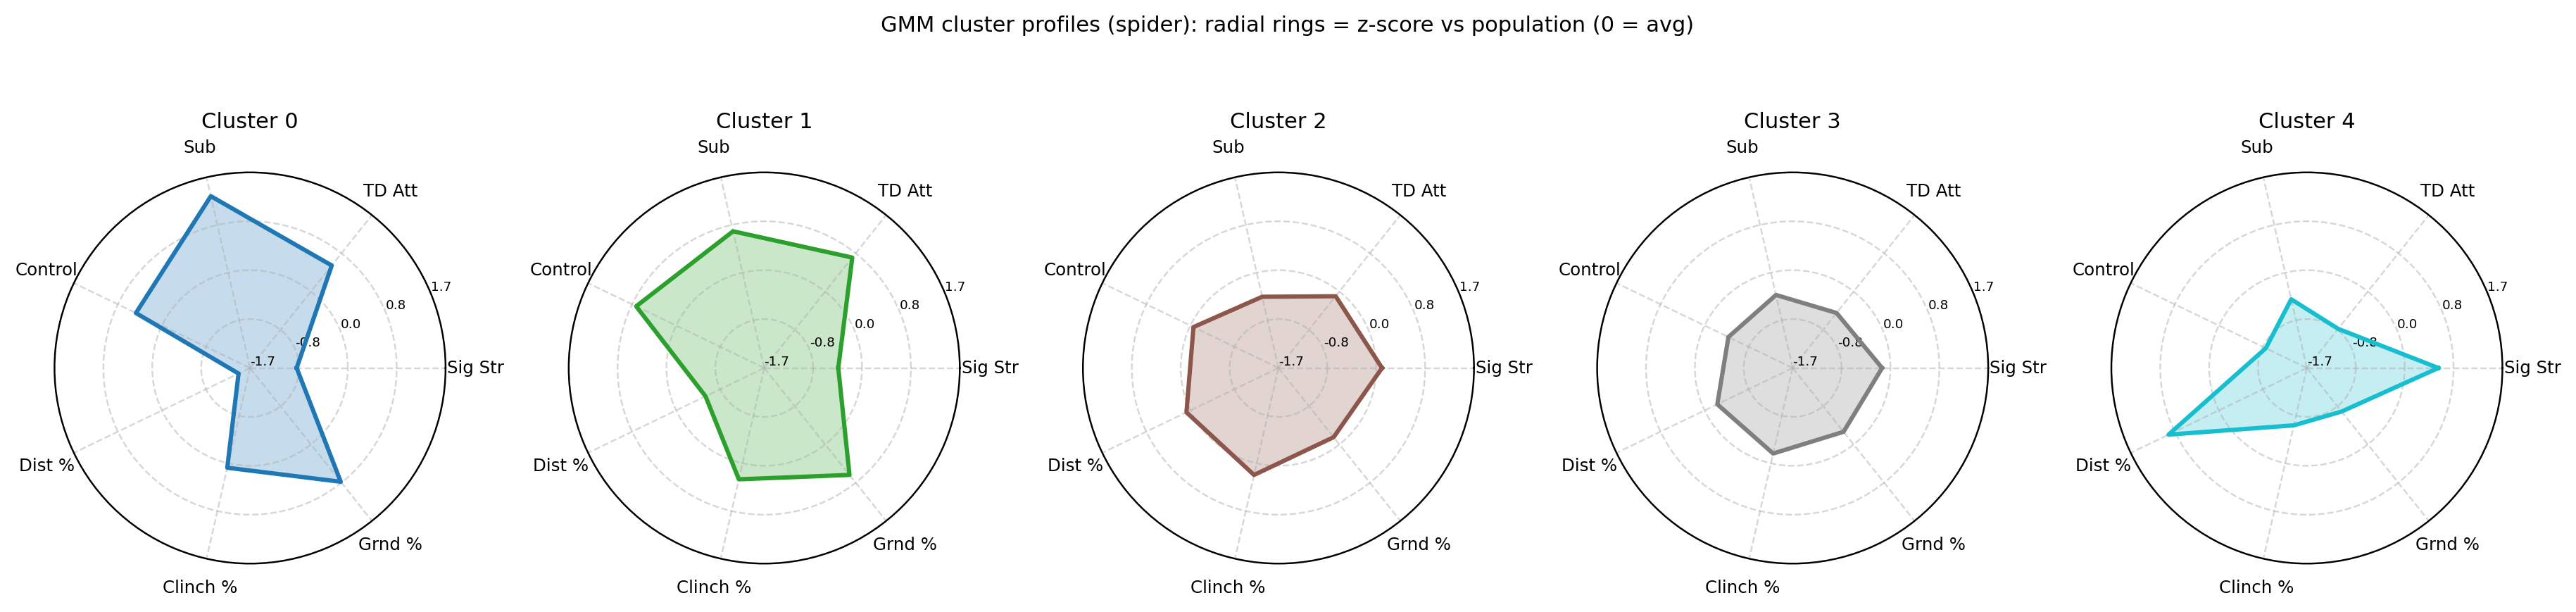
\includegraphics[width=0.88\textwidth]{gmm_profiles_k5.png}
\caption{Spider (radar) plots of centroid $Z$-score profiles for the \(K = 5\) Gaussian mixture: one panel per mixture component, common radial scale across panels, and ring labels read relative to the population mean (zero is average); submission-leaning grappler (0), active distance striker (1), low-activity (2), baseline generalist (3), takedown-heavy wrestler (4).  Source: notebook~10.}
\label{fig:gmm-profiles}
\end{figure}

\section{Qualitative champion check}\label{sec:champion-validation}

A silhouette score cannot tell a reader whether our representations
agree with how knowledgeable fans describe fighters.  To answer that
question we curate a panel of twenty-five UFC champions spanning
weight classes and eras, annotate each with a short expert label,
and check how they land in the autoencoder space
(Figure~\ref{fig:ae-champions}).  This is a face-validity check, not
a formal validation: the panel is small, hand-picked, and labeled
with informal expert intuition rather than tested against a
held-out outcome.

Three patterns emerge.  First, fighters described as
universally similar cluster together: Khabib Nurmagomedov, Islam
Makhachev, and Georges St-Pierre all land in Cluster~4 (takedown
wrestler) with Amanda Nunes and Randy Couture, and Max Holloway,
Jose Aldo, Conor McGregor, Israel Adesanya, and Alex Pereira all
land in Cluster~1 (distance striker).  Second, stylistically
distinct era-defining champions separate: Khabib, Holloway, and
Francis Ngannou fall into three distinct \(K = 5\) clusters.
Third, the Hybrid Score ranks generalists at the top of the
panel: Georges St-Pierre, Demetrious Johnson, Henry Cejudo, and
Daniel Cormier---the four fighters most routinely cited as the
sport's most complete generalists---sit in the upper quintile of
\(H(\pi)\), while Khabib (\(H \approx 0.07\)) and Ngannou
(\(H \approx 0.21\)) sit at the bottom.

\begin{figure}[ht]
\centering
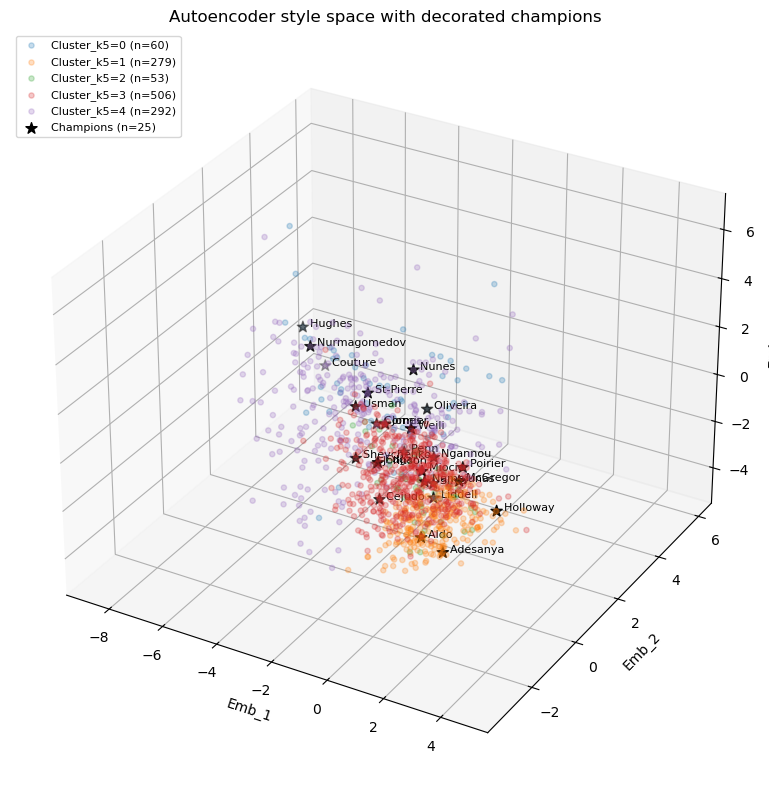
\includegraphics[width=0.88\textwidth]{ae_champions.png}
\caption{Three-dimensional autoencoder style space with twenty-five
annotated UFC champions, colored by \(K = 5\) hard assignment.  Khabib,
Makhachev, and GSP cluster with other wrestler-dominant fighters;
Holloway, Aldo, McGregor, Adesanya, and Pereira cluster with other
kickboxing-style strikers; generalists such as Jon Jones,
Volkanovski, Johnson, and Cejudo fall in the baseline cluster
between.  A companion text table mapping each named champion to
their \(K = 5\) cluster appears in Section~\ref{sec:champion-validation};
the labels in this 3D figure are intentionally compact and the
table is the canonical reference.  Source: notebook~25.}
\label{fig:ae-champions}
\end{figure}

\begin{table}[ht]
\centering
\caption{Champion-to-cluster mapping for the panel in
Figure~\ref{fig:ae-champions} (\(K = 5\) hard assignment).  Cluster
names follow Figure~\ref{fig:gmm-profiles}: 1 = active distance
striker, 3 = baseline generalist, 4 = takedown wrestler.}
\label{tab:champion-cluster-map}
\small
\begin{tabular}{ll}
\toprule
\(K = 5\) cluster & Champions in panel \\
\midrule
1: distance striker & Holloway, Aldo, McGregor, Adesanya, Pereira \\
3: baseline generalist & Jones, Volkanovski, Dillashaw, Cejudo, Johnson, \\
                       & Ngannou, Cormier, Cruz, Usman, Edwards, \\
                       & Poirier, Weili \\
4: takedown wrestler & Khabib, Makhachev, St-Pierre, Nunes, Couture \\
\bottomrule
\end{tabular}
\end{table}

Two observations are worth flagging for later chapters.  First, the
champion panel is dominated by Cluster~3: twelve of the twenty-five
champions sit there.  The modal archetype of a modern UFC champion
is not ``striker'' or ``wrestler'' but generalist.  Second,
the representation occasionally contradicts the fan label.
Ngannou---described by fans as a one-shot power puncher and
``expected'' to cluster with the strikers---lands in Cluster~3, likely because his fights end so quickly (average duration under six
minutes) that his per-minute striking and grappling rates regress
to the population mean.  This is an honest quirk of the feature
space: per-minute normalization is what makes the representation
comparable across career lengths, and the price we pay is that a
fighter whose identity is ``one KO per fight in the first round''
looks average on per-minute rates.

\section{Style-pair interactions and a first null result}\label{sec:heatmap}

With hard \(K = 5\) assignments in hand we tabulate the empirical win rate
$w_{ij}$ of Cluster~$i$ versus Cluster~$j$
(Figure~\ref{fig:style-heatmap}).  The heatmap is predominantly near
$0.5$: style alone is a weak unconditional predictor of the outcome,
consistent with the near-zero correlation of the ``style clash''
score with winning in \fref{fig:matchup-corr}.  Off-diagonal cells
display larger asymmetries, but many of those cells contain
only a handful of fights: the largest cell-level asymmetries
typically involve fewer than thirty bouts and would not survive
straightforward exact-test corrections at conventional levels.  The
heatmap should accordingly be read descriptively---as a compact
catalog of where the historical record is balanced and where it
appears to lean---and not as significance-tested evidence that one
style beats another.  Its row probabilities are attached to the
unified matchup table as the \(p_{\mathrm{heatmap},A}\) feature, where
they enter only as one column among many; the upset model
(Chapter~\ref{ch:upset}) finds the heatmap-minus-Vegas residual
below chance as a stand-alone signal, which is consistent
with the descriptive framing here.

\begin{figure}[ht]
\centering
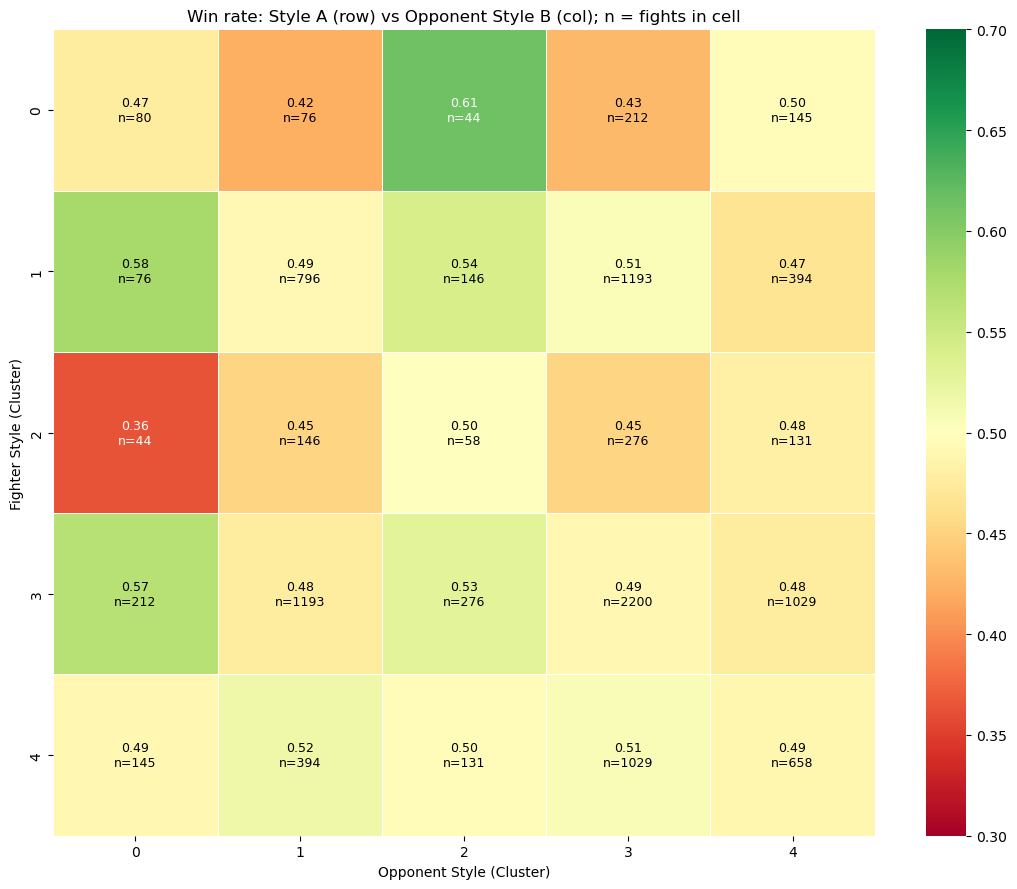
\includegraphics[width=0.78\textwidth]{style_heatmap.png}
\caption{Empirical win rate of \(K = 5\) style A (row) versus \(K = 5\)
style B (column), with fight counts per cell.  Predominantly near
$0.5$, consistent with style being a weak unconditional predictor;
many off-diagonal cells have small counts and should be read
descriptively.  Source: notebook~11.}
\label{fig:style-heatmap}
\end{figure}

A related and sharper test asks whether hybrid generalists
systematically outperform specialists because their opponents
``cannot game-plan'' against them.  Binning fighters into quintiles
of \(H(\pi)\) at \(K = 5\) (Figure~\ref{fig:hybrid-winrate}) produces no
bucket more than $1.5$ percentage points from $50\%$.  At the
population level the hybrid-beats-specialist hypothesis is
not supported.  The null is sharper than it looks: the same
question for how a fight unfolds and for when a favorite
is mispriced will return real, positive effects later, so what the
data rule out is specifically the claim that hybridness translates
into higher win rates in the aggregate---not the broader claim that
style is informative in the right task.

\begin{figure}[ht]
\centering
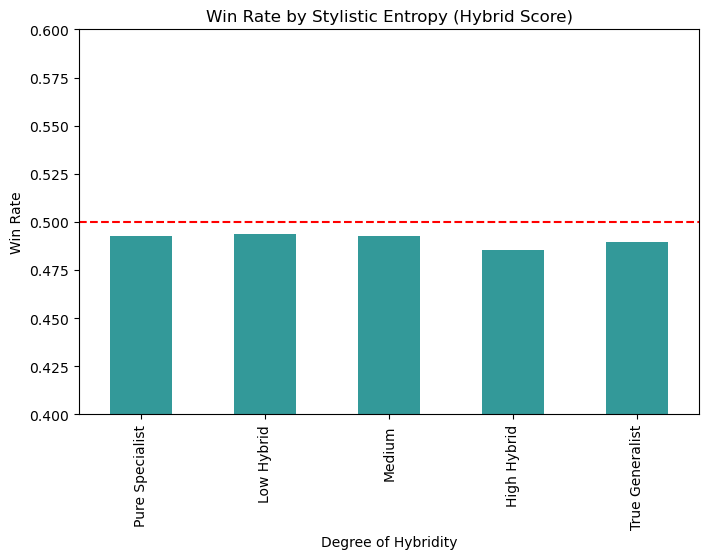
\includegraphics[width=0.70\textwidth]{hybrid_winrate.png}
\caption{Win rate by Hybrid Score quintile.  All five buckets lie
within $\pm 1.5$ percentage points of $50\%$; the
hybrid-beats-specialist hypothesis is not supported at the
population level.  Source: notebook~11.}
\label{fig:hybrid-winrate}
\end{figure}

% =====================================================================
\chapter{Does Style Predict Who Wins?}\label{ch:matchup}
% =====================================================================

The first of the thesis's three questions is whether style sharpens
prediction of who wins.  The answer developed here is: yes,
but at the margin.  A feature ablation across six model families along the non-market feature ladder lifts held-out AUC from $0.600$ to $0.670$
over a $Z$-score-delta baseline, and a Vegas-aware LR$+$HGB$+$RF stack
edges the de-vigged Vegas baseline on AUC, Brier, and log
loss when \(p_{\mathrm{vegas},A}\) is added as a fourth meta-input.  Neither result displaces the Vegas baseline; what they establish is
that style carries marginal predictive content beyond classical
features, and that the content survives when Vegas is already
present---the condition under which residual upset prediction in
Chapter~\ref{ch:upset} becomes possible.

\section{Model families and the ablation ladder}

Notebook~19 fits six supervised classifiers on the unified matchup
table---$\ell_2$-regularized logistic regression (LR); random
forests \citep{breiman2001random}; histogram-based gradient boosting
(HGB; \citealp{friedman2001greedy}; scikit-learn
\citealp{scikitlearn2011}); XGBoost \citep{chen2016xgboost}; LightGBM
\citep{ke2017lightgbm}; and a two-layer MLP trained in PyTorch
\citep{paszke2019pytorch} with Adam \citep{kingma2014adam}---as single-model candidates along a feature ablation ladder.
Hyperparameters are tuned on \texttt{val} and frozen before touching
\texttt{test}; non-probabilistic outputs are isotonically calibrated
\citep{zadrozny2002transforming} on \texttt{val}.
The final stack retains LR, HGB, and RF only: a logistic regression meta-learner on \texttt{val} combines their validation-set predicted probabilities, and the stacked output is isotonic-calibrated on \texttt{val}.
XGBoost, LightGBM (when available), and the MLP are evaluated in the bakeoff but are not included in this triplet stack.
The feature sets at each ablation rung, single-model family choices, stack composition, and calibration steps are all selected on \texttt{val} and frozen before any test-set evaluation; Notebook~19 implements this pipeline.

To quantify the marginal contribution of each feature family, every
model is trained on a sequence of nested feature sets that add one
group at a time.  Table~\ref{tab:ablation} reports held-out test
AUC and Brier for the best single learner at each step.  Two test
slices appear in the table: the full event-ordered test fold
($n = 1{,}850$) and the smaller Vegas-aligned subset ($n = 1{,}129$,
the rows for which a de-vigged moneyline is available).  We report
the non-market rows on both slices so the reader can separate
``feature gain'' from ``subset change.''

\begin{table}[ht]
\centering
\caption{Held-out test AUC and Brier along the feature-ablation
ladder; each row is the best single model at that step, selected on
validation AUC.  The first numeric block is the full test fold
($n = 1{,}850$); the second block restricts the same trained models
to the Vegas-aligned subset ($n = 1{,}129$); the bottom block adds
\(p_{\mathrm{vegas},A}\) as the market input.}
\label{tab:ablation}
\begin{tabular}{lccc}
\toprule
Feature set                & Subset & AUC   & Brier \\
\midrule
\multicolumn{4}{l}{Non-market features, full test (\(n = 1{,}850\))} \\
\texttt{z\_only} (LR)      & full   & 0.600 & 0.242 \\
\texttt{+gmm} (LR)         & full   & 0.629 & 0.243 \\
\texttt{+ae} (LR)          & full   & 0.636 & 0.243 \\
\texttt{+rolling} (HGB)    & full   & 0.664 & 0.239 \\
\texttt{+ratings} (HGB)    & full   & 0.670 & 0.236 \\
\texttt{full} (HGB)        & full   & 0.657 & 0.240 \\
\midrule
\multicolumn{4}{l}{Non-market features, Vegas-aligned subset (\(n = 1{,}129\))} \\
\texttt{full} (HGB)        & vegas  & 0.695 & 0.222 \\
Stack (LR+HGB+RF, no Vegas)& vegas  & 0.698 & 0.218 \\
\midrule
\multicolumn{4}{l}{Adding the market, Vegas-aligned subset (\(n = 1{,}129\))} \\
\texttt{full+vegas} (stack) & vegas & 0.775 & 0.192 \\
Vegas alone                 & vegas & 0.751 & 0.201 \\
\bottomrule
\end{tabular}
\end{table}

Along the non-market full-test ladder, validation-selected models raise AUC from
$0.600$ to a peak of $0.670$ at the \texttt{+ratings} rung; the final \texttt{full} row is slightly lower ($0.657$).
GMM posteriors ($+0.03$), autoencoder embeddings ($+0.01$), and rolling
pre-fight rates ($+0.03$) are the three non-trivial contributors;
physicals and weight-class one-hots add nothing further after
$Z$-scoring.  Restricting the same \texttt{full} HGB model to the
Vegas-aligned subset moves AUC from $0.657$ to $0.695$---a gain that
reflects subset composition rather than a feature change; the thesis does not attempt to decompose which rows drive that subset effect.  Adding \(p_{\mathrm{vegas},A}\) on top of the full
non-market block then moves AUC from $0.698$ (Stack without Vegas,
same subset) to $0.775$ (Stack$+$Vegas).  The reader who wants the
``feature-only'' improvement from non-market to Vegas-aware should
compare the two Vegas-subset rows in the middle and bottom blocks
($0.695\!\to\!0.775$ for HGB, or $0.698\!\to\!0.775$ for the
stack); the reader who wants the headline improvement over the
$Z$-score baseline should still use the full-test
$0.600\!\to\!0.670$ ladder figure (the peak at \texttt{+ratings}, not the final \texttt{full} row).

\section{Does the stack beat Vegas?}\label{sec:vegas-compare}

The comparison runs on the objective label \texttt{Win\_A} so no
circularity enters from the definition of ``favorite.''  The
Vegas-aligned test subset contains \(n = 1{,}129\) rows; both
models in the comparison are trained on the same (Vegas-aligned)
training rows and evaluated on the same test rows.

\begin{table}[ht]
\centering
\caption{Win-loss metrics on the Vegas-aligned held-out test subset
(\(n = 1{,}129\)); lower is better for Brier and log loss.  ``Stack''
is the LR$+$HGB$+$RF ensemble with a logistic meta-learner fit on
\texttt{val} followed by isotonic calibration on \texttt{val},
without Vegas, trained on Vegas-aligned training rows; ``Stack+Vegas'' is the same
stack with \(p_{\mathrm{vegas},A}\) added as a fourth meta-input.
Paired bootstrap (Stack+Vegas $-$ Vegas), $2{,}000$ resamples.}
\label{tab:vegas-compare}
\begin{tabular}{lccc}
\toprule
Model       & AUC     & Brier   & Log loss \\
\midrule
Vegas       & $0.751$ & $0.201$ & $0.588$  \\
Stack       & $0.698$ & $0.218$ & $0.626$  \\
Stack+Vegas & $0.775$ & $0.192$ & $0.562$  \\
\midrule
$\Delta$AUC      & \multicolumn{3}{l}{$+0.023$\ \ 95\% CI $[+0.001,\ +0.045]$,\ $p = 0.04$} \\
$\Delta$Brier    & \multicolumn{3}{l}{$-0.010$\ \ 95\% CI $[-0.018,\ -0.001]$,\ $p = 0.02$} \\
$\Delta$log loss & \multicolumn{3}{l}{$-0.025$\ \ 95\% CI $[-0.046,\ -0.004]$,\ $p = 0.01$} \\
\bottomrule
\end{tabular}
\end{table}

Stack+Vegas beats Vegas alone on all three metrics at \(p \le 0.05\),
with 95\% paired bootstrap CIs that exclude zero in every case.  The
effect is small but distinguishable from sampling noise.  Equally important,
the pure non-market stack (``Stack'') is worse than Vegas on
every metric ($\Delta$AUC $= -0.054$ with 95\% CI
$[-0.093,\ -0.017]$).  The positive result is therefore not ``style
beats the book on its own'' but the sharper claim that style and
the rolling pre-fight features together contribute information the
book does not already incorporate.  The reliability curves in
Figure~\ref{fig:reliability-vegas} show the same story
geometrically: \texttt{Stack+Vegas} tracks the diagonal more closely
than Vegas alone and attains lower Brier, log loss, and ECE, while
the Vegas-free models sit below the diagonal at short odds and above
it at long odds.  Grouped permutation importance on the stacked
model (reprised for the upset model in Chapter~\ref{ch:upset})
confirms that \(p_{\mathrm{vegas},A}\) is by far the single most
important column; among non-market features, the rolling pre-fight
rates and the autoencoder embedding are the two largest
contributors.

\begin{figure}[ht]
\centering
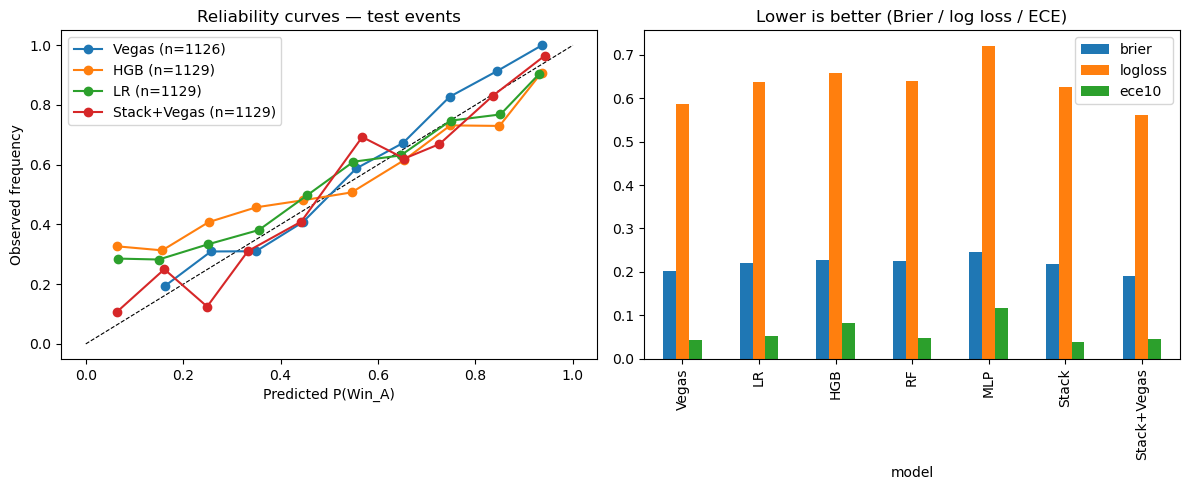
\includegraphics[width=0.95\textwidth]{reliability_vegas.png}
\caption{Left: reliability curves on the Vegas-aligned test subset
for Vegas, HGB (non-Vegas features), logistic regression (full), and
the stack with Vegas as a feature.  Right: Brier, log loss, and ECE.
\texttt{Stack+Vegas} tracks the diagonal most closely and attains
the lowest Brier, log loss, and ECE.  Legend $n$ is the full
Vegas-aligned test count; curve points omit probability bins with
fewer than five rows.  Source: notebook~20.}
\label{fig:reliability-vegas}
\end{figure}

On who wins, then, style is a supporting actor: it lifts the
feature-stack AUC by a few points above a $Z$-score baseline, is
strictly dominated by Vegas on its own, and beats Vegas only by a
margin whose CIs make it hard to dismiss but too small to overstate.
Combined with the hybrid-versus-specialist null of
Section~\ref{sec:heatmap}, the natural question is where, if
anywhere, style decisively matters.  The next two chapters argue
the answer is how the fight unfolds and when a
favorite is vulnerable.

% =====================================================================
\chapter{Does Style Predict How Fights Unfold?}\label{ch:dynamics}
% =====================================================================

If who wins is the hardest of the three questions, how
a fight unfolds is the richest: duration, method of victory, and
strike and grapple volume are all dimensions along which style can
leave a fingerprint.  This chapter reports two headline findings: a
hierarchical factorization of the method of victory, and the
thesis's cleanest positive style effect, found in the
\(K = 5\) GMM-posterior-divergence-to-finish-rate curve.  It closes with a brief check of continuous dynamics targets.

A flat six-way classifier over \{\texttt{A\_KO}, \texttt{A\_SUB},
\texttt{A\_DEC}, \texttt{B\_KO}, \texttt{B\_SUB}, \texttt{B\_DEC}\}
must jointly learn ``will there be a finish?'' and ``who finishes
whom?'' from a single softmax.  We instead factor the six-way problem into a binary finish head, a conditional finish-method head for KO versus submission among finished fights, and winner heads conditional on the relevant branch.  Schematically, the probability of an outcome is assembled from \(P(\mathrm{finish})\), \(P(\mathrm{method}\mid \mathrm{finish})\) for finished fights, and \(P(\mathrm{winner}\mid \mathrm{branch})\) for the relevant finish or decision branch.  We train one histogram-based gradient booster
\citep{friedman2001greedy} for each piece of this decomposition.  On the held-out
test slice the hierarchical model attains log loss $1.94$ versus
$2.15$ for the flat six-way HGB, a $10\%$ reduction.  The largest
per-cell improvement is on the rare submission classes, which is consistent with the structure allowing the model to borrow strength from
the common binary finish head rather than having to learn
submission-specific probabilities from a handful of examples.

The chapter's headline plot is the relationship between
\(K = 5\) GMM-posterior style divergence---the Euclidean
distance \(\lVert \pi_A - \pi_B \rVert_2\) between the two corners'
soft cluster posteriors---and the realized finish rate
(Figure~\ref{fig:style-divergence-finish}).  Across quintiles of
posterior divergence on fights with both posteriors observed, the
realized finish rate is $0.50$, $0.46$, $0.47$, $0.51$, and $0.56$
in quintiles 1 through 5; the top-quintile rate is roughly nine
percentage points above quintiles 2 and 3, and roughly six
percentage points above the bottom quintile.  The honest
interpretation is therefore not ``monotone in divergence'' (the
bottom four bins are noisy and roughly flat) but rather the
tail of stylistically mismatched fights finishes noticeably more
often---consistent with the intuition that the most decisive bouts happen
when one fighter's posterior over archetypes places mass far from
the other's.  The continuous autoencoder version of this analysis
on \(\lVert z_A - z_B \rVert_2\) produces a qualitatively similar
top-quintile lift; we report the GMM-posterior version because it is directly interpretable: the distance is measured between the fighters' soft archetype memberships.

As a sanity check on the non-trivial finish-rate pattern, binary
finish Brier on the test rows that have the full six-way
method-of-victory market available (\(n = 1{,}827\)) is $0.260$ for our
model and $0.351$ for \(p_{\mathrm{finish}}^{\mathrm{vegas}}\) derived
from those method props by proportional de-vigging
(Section~3.1).  The two numbers run on the same rows and the same
binary $y_{\text{finish}}$; the model's advantage on this metric is
not merely a recoverable function of moneyline odds.

\begin{figure}[ht]
\centering
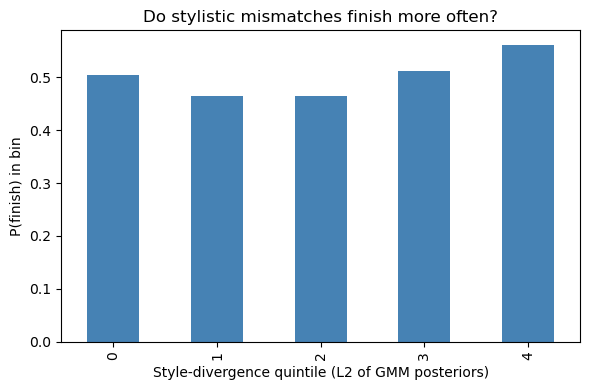
\includegraphics[width=0.70\textwidth]{style_divergence_finish.png}
\caption{Observed finish rate by quintile of \(K = 5\)
GMM-posterior style divergence \(\lVert \pi_A - \pi_B \rVert_2\) on
fights with both posteriors observed.  Quintile-wise realized
finish rates are $0.50,\ 0.46,\ 0.47,\ 0.51,\ 0.56$; the top
quintile sits roughly nine percentage points above the middle bins,
concentrated in the tail of maximally mismatched matchups.
Source: notebook~21.}
\label{fig:style-divergence-finish}
\end{figure}

Continuous dynamics targets split cleanly into predictable and
stubborn: takedowns (\(R^2 \approx 0.18\)) and submission attempts
(\(R^2 \approx 0.15\)) are meaningfully regressable on pre-fight
features, while striking totals (\(R^2 \approx 0.08\)) and fight
duration (\(R^2 < 0\) against a weight-class-mean baseline) are
dominated by round-level variance.  Grappling activity is a stable
career trait; striking totals are heavy-tailed in round-level shot
counts.  On how fights unfold, style is a first-class signal
wherever the dimension of variation is structural (finish rate,
method of victory, takedown volume) and a secondary signal wherever it is noise-driven (strike totals, duration). The next chapter asks
whether this same structural signal helps identify fights the market has mispriced, while keeping the betting interpretation economically and statistically honest.

% =====================================================================
\chapter{Does Style Help Catch Upsets?}\label{ch:upset}
% =====================================================================

Chapter~\ref{ch:matchup} established that a Vegas-aware stack edges
the de-vigged Vegas baseline by a small aggregate margin.  Chapter~\ref{ch:dynamics}
established that \(K = 5\) GMM-posterior divergence cleanly tracks
the realized finish rate, with the autoencoder version of the
divergence producing a qualitatively similar top-quintile lift.
The question for this chapter is
whether these two findings combine: does a Vegas-aware model that uses the
autoencoder embedding among its features systematically flag upset
candidates the market has mispriced---and if so, does the signal
carry economic content?  The answer is yes on the first half and
conditionally yes on the second; the conditions are spelled
out before any number is stated.

\section{Residual formulation and the signal check}

We train a HistGradientBoostingClassifier on the \texttt{full+vegas}
feature set to predict \texttt{Win\_A}, calibrate it with isotonic regression on \texttt{val}, and
score each test row by the residual
\[
r \;=\; p_{\mathrm{model}}(\mathrm{Win}_A \mid \mathrm{features}, p_{\mathrm{vegas},A}) \;-\; p_{\mathrm{vegas},A}.
\]
Positive $r$ means the model places more mass on corner A than the
market does.  The directional ``underdog-support'' score flips
sign when B is the favorite: $s = r$ if \(p_{\mathrm{vegas},A} < 0.5\),
else $s = -r$.  A bet is placed on the Vegas underdog whenever
\(s \ge \theta\).  On the full Vegas-aligned test slice, $s$ attains
ROC-AUC $0.588$ as an upset detector with a top-decile lift of
$1.56\times$ over the base rate.  The AUC is far from sufficient for a standalone betting strategy,
but it is sharp enough to motivate the thresholded ROI
simulation below.  Two baseline residuals---Elo-minus-Vegas and
heatmap-minus-Vegas---both score AUC below $0.50$, i.e.\ they are
directionally worse than random as upset classifiers, so $s$ is not
just a rediscovery of Elo or of the \(K = 5\) heatmap.

Figure~\ref{fig:perm-importance} reports grouped permutation
importance \citep{breiman2001random} on the trained upset model.
Among non-market groups, the autoencoder group is the largest
contributor: shuffling the three AE columns drops validation AUC by
more than any other group.  The rolling-rate group is next, matching
the Chapter~\ref{ch:matchup} ablation.  The GMM soft posteriors are
near zero, indicating redundancy with the smoother autoencoder for
this specific task.  These two roles are not in tension: the GMM
posterior carries non-redundant signal for finish rate
(Chapter~\ref{ch:dynamics}'s headline plot is on \(\lVert \pi_A - \pi_B \rVert_2\)), but for upset detection the relevant
question is how stylistically far apart two fighters are
after accounting for what the market already knows.  The
autoencoder's continuous \(\mathbb{R}^3\) space resolves
within-cluster style differences that the soft mixture collapses to
the same vertex region (Section~4.1's bridge), and that is the
content the upset model is rewarding.

\begin{figure}[ht]
\centering
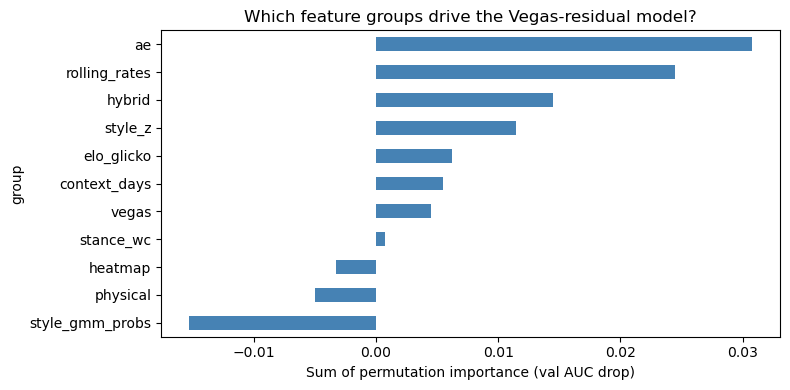
\includegraphics[width=0.80\textwidth]{upset_perm_importance.png}
\caption{Grouped permutation importance on the residual upset
model: validation-AUC drop when a feature group is shuffled.
Among non-market groups the autoencoder embedding (\texttt{ae}) is
the single largest contributor; GMM soft posteriors are negligible
for this specific task (cf.\ Chapter~\ref{ch:dynamics} where the
GMM posterior carries the finish-rate signal).
Source: notebook~22.}
\label{fig:perm-importance}
\end{figure}

\section{ROI with bootstrap intervals}

\paragraph{What the simulation is and is not.}  We treat the
ROI numbers below as evidence of residual market information
in the style-aware features---not as a deployable betting
strategy.  A deployable strategy would have to clear several bars
the simulation does not: (i) the payouts are de-vigged implied
probabilities, not tradable closing odds, so any real-money return
would be lower once the book's vig is re-applied; (ii) the
simulation does not model line movement between scrape time and
fight time, and it ignores book limits and stake-sizing; (iii) the
test window is a single $20\%$ event-ordered slice, not a
multi-year out-of-time forward test; (iv) the threshold \(\theta\)
was not pre-registered: we inspected several values on the
test set and report multiple in Table~\ref{tab:roi}; the headline
\(\theta = 0.15\) is the smallest grid value at which the bootstrap
CI excludes zero, and we therefore label the headline number
exploratory; (v) the upset model itself uses style features that
are static career-aggregate descriptors
(Section~\ref{sec:leakage-scope}), so the result reads more
naturally as ``does stable career-level style identity carry
non-market information'' than as ``does a strict pre-fight signal
beat the closing line.''  With those caveats firmly in front, the
flat-stake ROI simulation is reported as follows.  For every
test-slice row, bet one unit on the Vegas underdog whenever
\(s \ge \theta\), receive the de-vigged decimal payout on a win, and
lose the stake otherwise.  Paired-bootstrap $95\%$ CIs from
$2{,}000$ resamples are reported across the threshold grid in
Table~\ref{tab:roi}.

\begin{table}[ht]
\centering
\caption{Simulated flat-stake ROI of the $s = r$ upset policy on
the Vegas-aligned test slice, using de-vigged (not tradable)
implied prices.  $P(\mathrm{ROI} \le 0)$ is the empirical probability
of a non-positive resample ROI from $2{,}000$ paired bootstrap
draws.  \(\theta = 0.15\) is the headline threshold but was selected
post-hoc as the smallest grid value at which the CI excludes zero;
all four rows are reported so the reader can see the threshold
sensitivity.}
\label{tab:roi}
\begin{tabular}{cccccc}
\toprule
\(\theta\) & $n_{\text{bets}}$ & Hit rate & Obs.\ ROI & 95\% CI & $P(\mathrm{ROI} \le 0)$ \\
\midrule
$0.05$ & $674$ & $0.343$ & $+3.9\%$  & $[-7.8\%,\ +15.3\%]$ & $0.27$ \\
$0.10$ & $538$ & $0.349$ & $+9.4\%$  & $[-4.3\%,\ +23.1\%]$ & $0.10$ \\
$0.15$ & $411$ & $0.363$ & $+17.5\%$ & $[+1.5\%,\ +34.1\%]$ & $0.02$ \\
$0.20$ & $309$ & $0.369$ & $+23.4\%$ & $[+4.2\%,\ +43.8\%]$ & $0.01$ \\
\bottomrule
\end{tabular}
\end{table}

At looser thresholds (\(\theta \le 0.10\)) the bootstrap CI spans zero;
at \(\theta \ge 0.15\) the lower bound is positive, $P(\mathrm{ROI} \le
0)$ drops to about $2\%$ or below, and the hit rate rises from $0.34$ to $0.37$
in the expected direction.  The defensible
claim is that, for the question of when a favorite is vulnerable,
style is
the dominant non-market contributor to a residual detector, and the
detector produces a positive simulated return on a single held-out
window with paired-bootstrap CIs excluding zero at the two stricter
thresholds, \(\theta = 0.15\) and \(\theta = 0.20\); this is evidence of
residual market information rather than a deployable strategy.  A pre-registered
out-of-time test on 2025+ events with \(\theta\) locked on a
$2022$-vintage validation set is the next step
(Chapter~\ref{ch:conclusion}).

% =====================================================================
\chapter{Historical Upset Case Studies}\label{ch:cases}
% =====================================================================

This chapter is presented as illustrative rather than as a
validation set.  We did not score every upset in UFC history and
select the highest-residual five; we picked five canonical
moneyline upsets that fans and commentators recurrently invoke and
asked whether the framework, applied prospectively, produces
residuals consistent with what Chapter~\ref{ch:upset}'s threshold
policy would have bet.  Selection is by historical fame, and the
panel is small enough that a single dramatic mismatch would skew
the picture; the residuals below should be read as concrete
worked examples of the population-level result, not as independent
out-of-sample evidence.

Notebook~24 applies the unified feature table to five canonical
upsets, fitting a fresh \texttt{HistGradientBoostingClassifier} on
every fight strictly preceding each event's date so that each
prospective \(p_{\mathrm{model}}\) is leakage-free at the supervised
level; the style features that this prospective model consumes are,
as elsewhere in the thesis, the static career-aggregate
descriptors of Section~\ref{sec:leakage-scope}, which inherit the
same retrospective scope.  The case-study residuals are reported in
Table~\ref{tab:cases}.

\begin{table}[ht]
\centering
\caption{Five canonical UFC upsets, listed by event.  \(p_{\mathrm{vegas}}\)
and \(p_{\mathrm{model}}\) are reported on the eventual winner where
available; \(r = p_{\mathrm{model}} - p_{\mathrm{vegas}}\) is the
winner-oriented residual that Chapter~\ref{ch:upset}'s threshold
policy would have seen.  Each \(p_{\mathrm{model}}\) is fit by a
symmetry-augmented HGB on all fights strictly preceding the event
date.  A residual of $\ge 0.15$ would have triggered a bet under
the \(\theta = 0.15\) policy of Chapter~\ref{ch:upset}; this is the
same exploratory threshold flagged in Section~\ref{sec:repro}.}
\label{tab:cases}
\small
\begin{tabular}{lll cccc ll}
\toprule
Event (yr) & Winner & Loser & \(p_{\mathrm{vegas}}\) & \(p_{\mathrm{model}}\) & \(r\) & \(\lVert z_A - z_B \rVert_2\) & $k_W$ & $k_L$ \\
\midrule
UFC 69 (2007)  & Serra     & St-Pierre & ---    & $0.05^\dagger$ & ---    & $4.07$ & $4$ & $4$ \\
UFC 173 (2014) & Dillashaw & Barao     & $0.12$ & $0.32$         & $+0.20$ & $1.77$ & $3$ & $1$ \\
UFC 193 (2015) & Holm      & Rousey    & $0.15$ & $0.59$         & $+0.43$ & ---    & $1$ & ---  \\
UFC 269 (2021) & Pena      & Nunes     & $0.12$ & $0.38$         & $+0.26$ & $3.49$ & $4$ & $4$ \\
UFC 278 (2022) & Edwards   & Usman     & $0.27$ & $0.42$         & $+0.15$ & $3.33$ & $3$ & $3$ \\
\bottomrule
\end{tabular}

\smallskip
{\footnotesize $^\dagger$~\(p_{\mathrm{model}}\) for Serra; Vegas
moneylines are unavailable for UFC~69 in the Kaggle scrape so no
residual is reported.  ``---'' for the Holm/Rousey row marks
fighters whose career aggregates were too thin for a stable
autoencoder embedding and a \(K = 5\) assignment at the time the
static style table was built (Rousey appears in the matchup table
without an embedding or hard cluster).  Because both the
autoencoder divergence and the loser's cluster are missing, this
row should not be read as evidence of a cross-cluster mismatch
inside the framework---it is an honest gap in the static style
table.}
\end{table}

Three readings of Table~\ref{tab:cases} are worth pulling out, each
matched to a specific claim from earlier chapters.

\paragraph{Cross-cluster style mismatches (Dillashaw/Barao).}
Dillashaw (Cluster~3, baseline generalist with striking-heavy
rolling rates) and Barao (Cluster~1, active distance striker) are
the only pair in the panel whose hard \(K = 5\) assignments differ and
whose cluster-pair label is reported by the framework.  The
residual on the eventual winner, $+0.20$, exceeds the
\(\theta = 0.15\) threshold of Chapter~\ref{ch:upset} and is the
second-largest in the table.  Holm/Rousey is excluded from this cross-cluster reading for the missing-style-feature reason noted in Table~\ref{tab:cases}.

\paragraph{Within-cluster hidden mismatches (Edwards/Usman,
Pena/Nunes).}  More striking for the thesis's central argument are
the two cases whose hard \(K = 5\) assignments agree: Edwards
and Usman are both Cluster~3, and Pena and Nunes are both
Cluster~4.  A framework that relied on discrete archetypes alone
would describe these as same-style matchups and see no stylistic
asymmetry.  The continuous autoencoder embedding disagrees:
Euclidean divergences of $3.33$ and $3.49$ in \(\mathbb{R}^3\) sit in
the top quintile of the entire dataset, and the residuals on the
eventual winners---$+0.15$ and $+0.26$---both clear the
exploratory threshold.  These two cases, more than any cross-cluster
pair in the panel, illustrate the bridge from
Section~4.1: the soft mixture collapses two within-cluster fighters
to similar vertices on the simplex, while the autoencoder resolves
the within-cluster gap that the upset model is rewarding.

\paragraph{Pre-odds historical (Serra/St-Pierre).}  UFC~69 predates
reliable Kaggle moneyline coverage, so no residual is computable.
Our prospective model fit on all prior UFC fights assigns Serra only
a $5\%$ chance---the framework agrees with the contemporaneous
near-unanimous expectation of a St-Pierre win.  Serra's subsequent
first-round KO is a variance event the pre-fight features cannot
have predicted, and the framework correctly does not pretend
otherwise.

Taken together, the five rows give a concrete illustration of the
population-level ROI result of Chapter~\ref{ch:upset}: all four
cases for which a residual is computable clear \(\theta = 0.15\) on
the eventual winner, and the two within-cluster pairs illustrate
the continuous-over-discrete claim of Section~4.1 in the most
concrete form the thesis can offer.  The honest reading is illustrative, not
confirmatory: the panel was selected by fame, the missing values on
Holm/Rousey limit the cross-cluster story, and the panel is tiny
relative to the full historical UFC record.

% =====================================================================
\chapter{Discussion and Conclusion}\label{ch:conclusion}
% =====================================================================

The three empirical chapters answer the thesis's three questions
with answers of visibly different strength.  Who wins is the
hardest question and the one where style helps least: the non-market ablation lifts held-out AUC by a few points above a $Z$-score baseline, and the Vegas-aware LR$+$HGB$+$RF stack edges the de-vigged Vegas baseline by a small margin once \(p_{\mathrm{vegas},A}\) is added as a meta-input, with a paired null result on
hybrid-versus-specialist win rates sharpening the picture.
How fights unfold is where style becomes a first-class
signal: top-quintile \(K = 5\) GMM-posterior style divergence is associated with a realized finish rate roughly nine percentage points above the middle bins (the thesis's cleanest
positive style effect), and a hierarchical method-of-victory
decomposition cuts six-way log loss by $\sim 10\%$.  The upset task is where style carries the most practical
weight: the autoencoder embedding is the largest non-market
contributor to a residual upset detector, and an exploratory de-vigged
flat-stake policy returns a positive simulated ROI on a single
$20\%$ test window with a paired bootstrap CI that excludes zero
under the exploratory, post-hoc \(\theta = 0.15\) threshold.  The single-sentence
summary is that style, learned from career-level fighter
profiles, contains non-market predictive information about MMA
outcomes, especially fight dynamics and residual upset detection---a
more specific and testable version of ``styles make fights'' than
the cliché usually conveys, and not the stronger claim that the
model definitively beats the betting market in deployable practice.

\paragraph{Limitations.}  Three limitations shape how far these
results carry.  First, the UFCStats scrape omits non-UFC fights, so
extensive pre-UFC records---common for championship entrants---do
not enter our rolling aggregates, and Vegas coverage is partial and
skewed to recent events, so every Vegas-feature result is
restricted to a subset.  Second, the GMM posteriors and the
autoencoder embedding are fit on career-aggregate fighter profiles
(Section~\ref{sec:leakage-scope}) and therefore represent
style-as-identity rather than a strict pre-fight signal: fighters
whose styles change mid-career are modeled as stationary and
regress toward whichever archetype dominates their aggregate
record, which likely flattens the hybrid-versus-specialist test of
Chapter~\ref{ch:style}; the prospectively defensible block is the
rolling rates and the rating systems, and the deployable extension
of the style block is to refit the GMM and autoencoder on
expanding-window pre-fight statistics so that each fighter's
embedding at time $t$ uses only fights $<t$.  Third, the test slice
is a single $20\%$ event-ordered window rather than a multi-year
out-of-time test; the ROI simulation uses de-vigged implied
probabilities and ignores line movement, book limits, and stake
sizing, and \(\theta = 0.15\) was not pre-registered.

\paragraph{The most valuable single extension} is therefore a
pre-registered out-of-time test: refit the entire pipeline using
only events through 2022, lock \(\theta\) on \texttt{val} in advance,
swap the static GMM/autoencoder for an expanding-window pre-fight
fit so the style features at fight $t$ use only fights $<t$, and
evaluate the residual upset policy on $2023$ and $2024$ separately.
If the upset ROI survives that test, the framework moves from
exploratory statistical evidence toward a candidate deployable signal, though a real betting strategy would still require tradable odds, vig, line movement, and limit constraints.  Complementary directions are quantile
regression for the heavy-tailed dynamics targets; sequence models
of style evolution---a first pass with a Siamese GRU
\citep{bromley1994signature,cho2014learning} over the last eight
pre-fight rounds did not beat the HGB baseline (test AUC $0.58$
versus $0.65$), likely a sample-size issue that incorporating non-UFC history
could address; and a causal pass at the style-pair heatmap of
Section~\ref{sec:heatmap} that disentangles style from correlated
attributes (reach, camp, age cohort) via matching or
instrumental-variable designs to sharpen claims about why
certain styles beat certain others.  The contribution of this
thesis across all three is a compact, leakage-scoped style
representation that carries measurable non-market information about the
parts of MMA the cliché usually gets wrong.  Code and artifact layout are in \url{https://github.com/Jaaxe/ufc-matchup-dynamics} (\texttt{README.md}, \texttt{run\_pipeline.py}).

\clearpage\singlespacing

\bibliography{references/Bibliog,references/references}


\end{document}
